\chapter{State of the Art}
\label{chap:state-of-the-art}

\lettrine[lines=3, findent=3pt, nindent=0pt]{T}{his} chapter rounds out the theoretical background and technologies used in the project and discussed in the following: beginning with how network traffic is made ad how to characterize malicious activities, will then be discussed Software Defined Networking as an industry standard and then \gls{ml} will be introduced, with particular emphasis on Intrusion Detection applications. The reader should here be provided with sufficient knowledge to understand chapters \ref{chap:methodology}, \ref{chap:results} and \ref{chap:conclusions}.

%----------------------------------------------------
% NETWORK TRAFFIC
%----------------------------------------------------

\section{Network Traffic}
\label{sec:network-traffic}

\textit{Network Traffic} is the amount of data that passes through a network at a given time, and it represents the starting point to the project. \\ Network architecture was thought to be modular and explicit, to ensure that modifications made to a single component were transparent to the rest of the system. This modularization is represented by \textit{network protocols} being separated into different layers: each layer has a precise task. In 1960s the \textit{U.S. Department of Defense} designed the \textit{TCP/IP} model, which is now the \textit{de facto} standard for protocols stack. Network security should be addressed at each TCP/IP network layer for different vulnerabilities and attack types \cite{Zaman2009}.

\begin{figure}[h!]
    \centering
    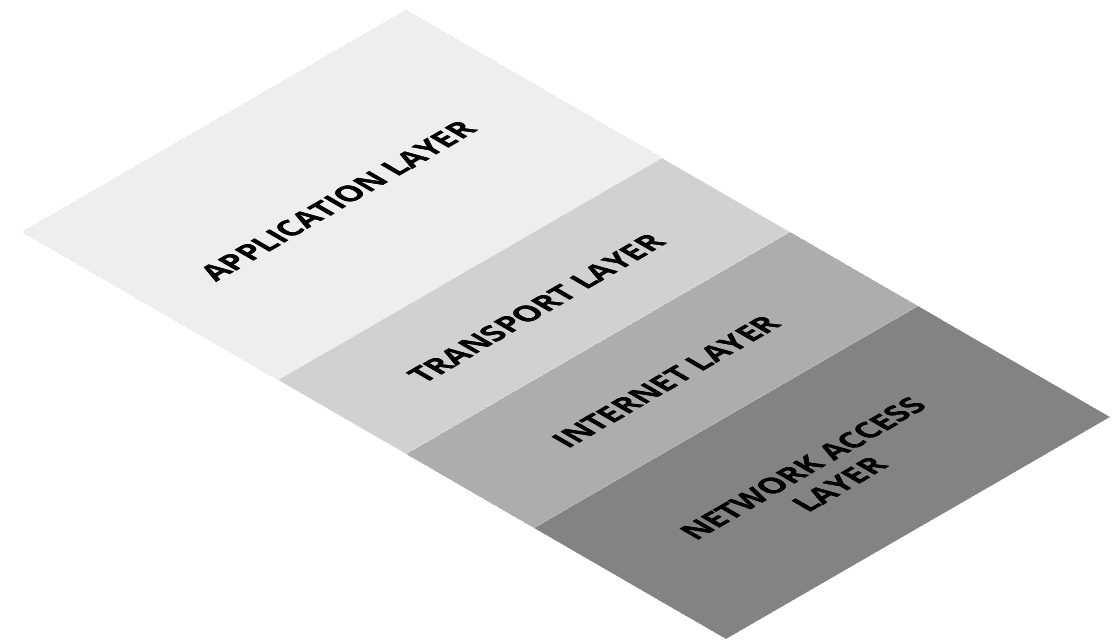
\includegraphics[scale=0.25]{assets/figures/chapter2/TCP_IP Stack.png}
    \caption{Internet protocol suite: TCP/IP Stack}
    \label{fig:TCP/IP-stack}
\end{figure}

\noindent TCP/IP stack is composed of 4 layers, representing from the physical connection (\textit{Network Access Layer}) to the user interface (\textit{Application Layer}). The most relevant layer for this project is the third one: \textit{Transport Layer}, also called \textit{Host to Host Layer} is responsible for end-to-end communication and error-free delivery of data. It shields the upper-layer applications from the complexities of data. The main protocols used in this layer are:

\begin{itemize}
    \itemAR \gls{tcp}: provides reliable and error-free communication between end systems. It also has acknowledgement features and a flow control system. This protocol has a lot of overhead due to its features \cite{Kurose2012};
    \itemAR \gls{udp}: unlikely \gls{tcp}, this protocol doesn't ensure a reliable connection between points, but it is very cost effective and lightweight \cite{Kurose2012}.
\end{itemize}
Network packets are encapsulated in either a \textit{TCP segment} or a \textit{UDP datagram}. Another relevant protocol that will be used is \gls{icmp}, belonging to the second layer (\textit{Internet Layer}): it is responsible for providing hosts with information about network problems. Because of the particular design of network architecture, in which one layer acts as an intermediate between the layer above and the one below, when trying to characterize the traffic, looking only at these latter protocols can be sufficient \cite{Iglesias2015}.

%----------------------------------------------------
% TRAFFIC MONITORING
%----------------------------------------------------

\subsection{Network Monitoring}
\label{subsec:network-monitoring}

\textit{Network monitoring} is becoming more and more important in the modern era, however, with new technologies and high traffic speed it is essential to manage in an efficient and scalable way the available resources. Network monitoring allows to know instantaneous state and long term trends of a network infrastructure. This practice can be either active or passive; the latter will be considered in this project. The process of network monitoring can be divided in two major steps: \textit{traffic duplication} and \textit{analysis}. A comprehensive overview of network monitoring approaches can be found in \cite{Svoboda2015}.

\subsubsection{Traffic Duplication}
\label{subsubsec:traffic-duplication}

In this stage the network traffic is duplicated from the main line, so the copy can be analyzed afterwards. There are two methods for this operation: \textit{inline} or \textit{mirroring} \cite{Svoboda2015}. The former can take place inserting a duplication device in link; on the other hand, the latter uses a built-in feature of the router or switch. Traffic duplication can be divided into:
\begin{itemize}
    \itemAR \textit{Port Mirroring}: as mentioned above, this is a functionality usually available in enterprise-oriented gear. This procedure consists, as the name suggests, in mirroring the traffic passing through selected ports, to others. Both directions of the monitored link are transmitted in one direction over the \textit{mirror port}, and this leads to its main downside: a full-duplex traffic is transmitted in one direction over the one port only: that is up to twice the bandwidth of a single port (considering only two ports being serviced by the switch), with consequent \textit{congestion} and \textit{packet drops}. It is now clear that port mirroring isn't scalable, and so will not be considered for the project;
    \itemAR \gls{tap}: a \gls{tap} is a packet capture device positioned in inline mode. This particular kind of device is placed between the split part of a line and duplicates the traffic. There are different types of \glsplural{tap}, depending on the medium of which the line is made: copper, fiber, \textit{virtual}. The downside of this approach is that introduces a point of failure in the physical line, and in some cases it can weaken the signal;
    \itemAR \textit{Bypass} \gls{nic}: This is also defined as a \textit{TAP-like setup}. It integrates traffic duplication with traffic analysis: a computer with two \glsplural{nic} is used to intercept the traffic of a split line; the interfaces are configured in software in \textit{bridge mode} (passing all the traffic through without manipulating it). This allows the computer to observe the traffic, similarly to a \gls{tap} and, as the above mentioned methodology, introduces a point of failure in the network, but has the advantage of being more flexible. It can also be realized using consumer-grade equipment.
\end{itemize}

\subsubsection{Traffic Analysis}
\label{subsubsec:traffic-analysis}

There are different approaches to traffic analysis, but all of them rely on \textit{Packet Capture}. This can be intended in two different manners: packet capture as a \textit{Packet Duplication Method} consists in capturing network traffic from an observation point; the captured data can then be saved (commonly) to a \gls{pcap} file. Packet capture as a \textit{Network Monitoring Approach} is composed of two steps: creating the \gls{pcap} file and then performing a network analysis on said data. An \gls{ids} can be considered as a complicated automated system. One of the main advantages, that can also represent a drawback is the interactivity of this method: full network data is accessible for free viewing in a second time, the problem is that the approach doesn't scale when dealing with large amounts of data \cite{Svoboda2015}. Traffic capture and analysis can be seen as separate processes, or can be integrated in pipeline. The main approaches to traffic analysis are: \textit{packet inspection} and \textit{flow-based characterization}. The first one consists of inspecting each network packet; it is very resource consuming and not always allowed since the payload can be encrypted. On the other hand, the second one is less precise, but much more cost effective and lightweight \cite{Alaidaros2017}. Machine learning methodologies can improve the detection rate of \textit{flow-based characterization} \cite{Iglesias2015}: this makes it a reliable go-to.

\begin{itemize}
    \itemAR \gls{dpi}: this technique consists in seeing the payload of \glsxtrshort{ip} packets. \gls{dpi}-based analysis can either be \textit{pattern matching} or \textit{event-based}. The former involves searching through full network data for known sequences of bytes. This can easily become a problem when dealing with large amounts of data, or complicated decision logic. This approach is slow and most of the times requires \glsxtrshort{fpga} hardware acceleration to handle the traffic throughput. \textit{Snort} \cite{SnortWebsite} and \textit{Suricata} \cite{SuricataWebsite} are implementations of pattern matching \gls{dpi}. On the other hand, event-based analysis relies on processing packets into events, that are then processed by scripts. Zeek \cite{ZeekWebsite}, formerly known as Bro, uses an event-based architecture;
    \itemAR \textit{Flow Observation}: this is a different approach to traffic analysis, that uses only the information contained in the packets' headers, not in the payload. This information is aggregated into \textit{flows}, which are defined in \cite{RFC7011} as \textit{`[...] a set of packets or frames passing an Observation Point in the network during a certain time interval. All packets belonging to a particular Flow have a set of common properties'}. To distinguish one flow to the other a 5-tuple consisting of \textit{source ip}, \textit{destination ip}, \textit{source port}, \textit{destination port} and \textit{protocol} is used. This architecture has several advantages: it is much more cost effective than the other methods both in terms of storage and performance. Another strong point of flow observation is privacy, in fact only aggregated metadata about the traffic is stored.
\end{itemize}

\noindent Flow observation is what will be used in this project, considering its scalability with high speeds, its optimization in terms of storage and also taking into account modern concerns about privacy. \\ This architecture is composed of five steps:

\begin{enumerate}
    \item \textit{Observation}: gathering information about network traffic;
    \item \textit{Metering}: this process identifies flows and calculate their statistics. From this point the original packet is not needed anymore;
    \item \textit{Export}: after a certain period of time the processed flows are exported;
    \item \textit{Collector}: in this stage metered flows are stored in order to be analyzed;
    \item \textit{Analysis}: flows are analyzed using, in this case, \gls{ml}.
\end{enumerate}

\noindent In the next sections \ref{subsec:traffic-characterization} and \ref{subsec:malicious-traffic} steps 2 and 5 will be clarified.

%----------------------------------------------------
% TRAFFIC CHARACTERIZATION
%----------------------------------------------------

%See paper \cite{Iglesias2015}, \cite{Sharafaldin2019} and \cite{icissp17} and \cite{Xu2017} and \cite{Dainotti2006} and \cite{Wijesinghe2015}

\subsection{Traffic Characterization}
\label{subsec:traffic-characterization}

Anomaly detection in communication networks provides the basis for uncovering misconfigurations, network failures and potential threats. Resource and time constraints create the need of restricting to a limited number of features the traffic characterization and task detection. Limiting the resources spent for the observation and the analysis of such data, also improves the quality of the detection, since trivial and redundant information will not be considered. In \cite{icissp17} and \cite{icissp18} \textit{time-related} features are suggested to characterize traffic with ease:
\begin{itemize}
    \itemAR \textit{Active}: duration of sending packets before idle;
    \itemAR \gls{biat}: time between two packets sent backward;
    \itemAR \textit{Duration}: duration of the considered flow.
    \itemAR \gls{fbpsec}: bytes sent per second in either direction;
    \itemAR \gls{flowiat}: time between two packets sent in either direction; 
    \itemAR \gls{fppsec}: packets sent per second in either direction;
    \itemAR \gls{fiat}: time between two packets sent forward; 
    \itemAR \textit{Idle}: amount of time the flow was idling before becoming active;
\end{itemize}
For all the features also the respective mean, minimum, maximum and standard deviation are calculated and so the above bullet list really represents groups of features\footnote{See appendix \ref{app:net-features}}.

%----------------------------------------------------
% MALICIOUS TRAFFIC
%----------------------------------------------------

\subsection{Malicious Network Traffic}
\label{subsec:malicious-traffic}

An \textit{intrusion} can be defined as an attempt to access information about computer systems or to damage system operation in an illegal or unauthorized manner \cite{Liu2019}, hence it will be considered \textit{malicious traffic} the entirety of network traffic generated by such operations. \\
The classes of malicious traffic analyzed in this work are the following:

\begin{itemize}
    \itemAR \textit{Botnet}: a botnet is a number of Internet connected devices, used to perform various tasks, from stealing data, to spam, or to practice \gls{ddos} attacks. Automated infection tools can also be used to scan for and compromise vulnerable zombie systems \cite[p.~250]{Sharafaldin2019} and \cite{icissp18};
    \itemAR \textit{Bruteforce}: this kind of attack is one of the most popular and it can be used to guess passwords or \glsxtrshortpl{url} (in order to discover hidden contents in web applications). It can be defined as an hint and try attack, that corresponds of trying every possible key on a piece of ciphertext until an intelligible translation into plaintext is obtained \cite[p.~43]{Sharafaldin2019} and \cite{icissp18};
    \itemAR \gls{xss}: this kind of vulnerability can typically be found in web applications. An \gls{xss} attack consist of injecting client-side scripts into \glsxtrshort{html} content of web pages, that can be viewed by other users and aims to gain elevated access privileges to sensitive data belong- ing to other sites \cite[p.~387]{Sharafaldin2019};
    \itemAR \gls{dos}: the objective of this attack is to exhaust some critical resources associated with the target service, denying or preventing legitimate users to access the system or the network \cite[p.~241]{Sharafaldin2019};
    \itemAR \gls{ddos}: unlike the previous type of attack, the incoming traffic flooding the victim is obtained from many different sources. This effectively makes it impossible to stop the attack simply by blocking a single source and guarantees much more bandwidth to the attacker \cite[p.~241]{Sharafaldin2019};
    \itemAR \textit{Heartbleed}: this particular attack exploits a bug in the OpenSSL cryptography library, widely used implementation of the \gls{tls} protocol. It was discovered in 2014 and allowed to expose significant amounts of memory on the vulnerable systems \cite{Carvalho2014}, \cite[p.~706]{Sharafaldin2019}, \cite{icissp18} and \cite{Stallings2014};
    \itemAR \textit{Port Scanning}: this occurs when an attacker sends probe packets to gather intelligence information about the infrastructure, based on the responses received \cite{icissp18};
    \itemAR \gls{sqli}: it is one of the most prevalent and dangerous network-based security threats that uses malicious database queries to extract bulk data from the latter; this can occur, for example, through badly projected forms on web pages \cite[p.~163]{Sharafaldin2019}.
\end{itemize}
The purpose of this section was not to provide a comprehensive list of all possible network violations, rather to point out some of the most important known vulnerabilities and methodologies, which are contained in the dataset\footnote{See section \ref{subsec:datasets-for-evaluation}} used for the evaluation.

%----------------------------------------------------
% SOFTWARE DEFINED NETWORKING
%----------------------------------------------------

\subsection{Software Defined Networking}
\label{subsec:sdn}

Follows a brief introduction on \gls{sdn} as an industry standard, now widely available also in consumer-grade equipment. \gls{sdn} technology is an approach to network management that enables dynamic and efficient network configuration with the aim of improving network performance and monitoring. It was first issued by the \gls{ietf} in the 2000s and since its refinement it was associated with \textit{OpenFlow protocol}, although nowadays it isn't anymore an exclusive solution. In the \gls{sdn} paradigm the network architecture consists fo three planes: \textit{data plane} (that forwards traffic according to the decisions made by the control plane), \textit{control plane} (that decides how to handle network traffic) and \textit{application plane} \cite{Kreutz2015}.

\begin{figure}[h!]
    \centering
    \begin{tikzpicture}[scale=.45,every node/.style={minimum size=1cm},on grid]
            
        %slanting: production of a set of n 'laminae' to be piled up. N=number of grids.
        \begin{scope}[
                yshift=-83,every node/.append style={
                yslant=0.5,xslant=-1},yslant=0.5,xslant=-1
                ]
            % opacity to prevent graphical interference
            \fill[white,fill opacity=0.9] (0,0) rectangle (5,5);
            \draw (2.4,2.5) node {\fontsize{40}{40} \faRandom};
            \draw[black,very thick] (0,0) rectangle (5,5);%marking borders
            %Idem as above, for the n-th grid:
        \end{scope}
            
        \begin{scope}[
            yshift=0,every node/.append style={
                yslant=0.5,xslant=-1},yslant=0.5,xslant=-1
                         ]
            \fill[white,fill opacity=.9] (0,0) rectangle (5,5);
            \draw[black,very thick] (0,0) rectangle (5,5);
            \draw (2.4,2.5) node {\fontsize{40}{40} \faServer};
        \end{scope}
            
        \begin{scope}[
            yshift=90,every node/.append style={
            yslant=0.5,xslant=-1},yslant=0.5,xslant=-1
                         ]
            \fill[white,fill opacity=.9] (0,0) rectangle (5,5);
            \draw (2.4,2.5) node {\fontsize{40}{40} \faTv};
            \draw[black,dashed] (0,0) rectangle (5,5);
        \end{scope}
    
        %putting arrows and labels:
        \draw[-latex,thick] (6,4) node[right]{$\mathsf{Control\; Plane}$}
             to[out=180,in=90] (3.5,2.5);
    
        \draw[-latex,thick](6,1)node[right]{$\mathsf{Data\; Plane}$}
             to[out=180,in=90] (3.5,-0.5);
    
        \draw[-latex,thick](6,7)node[right]{$\mathsf{Application\; Plane}$}
            to[out=180,in=90] (3.5,5.5);
        
    \end{tikzpicture}
    \caption{\gls{sdn} paradigm}
    \label{fig:sdn-paradigm}
\end{figure}
\noindent The bottom plane is made up of \gls{sdn}-enabled switches, that send routing request to the above plane, instead of calculating routing rules by themselves when receiving new \textit{flows}, then the control plane calculates paths for the requests and assigns the routing rules in compliance with the applications in the top plane \cite{Xu2017}. The \textit{controller} exercises direct control over the state in the data plane elements via well-defined \glsplural{api}, such as OpenFlow. An OpenFlow switch has one or more tables of packet-handling rules (flow table). Each rule matches a subset of the traffic and performs certain actions on the traffic. Depending on the rules installed by a controller application, an OpenFlow switch can - instructed by the controller - behave like a router, switch, firewall, or perform other roles and this leads to fault tolerance and scalability \cite{Lantz2015}. This is what makes this technology so convenient.

%----------------------------------------------------
% SDN CONTROLLER
%----------------------------------------------------

\subsubsection{SDN Controller}
\label{subsubsec:sdn-controller}

%See paper \cite{Zhu2019} and \cite{Bondkovskii2016} \\
The \textit{controller} is the fundamental element used for all operations of data plane management. Hence, the performance and capabilities of the controller itself are extremely important and in this project its \glsplural{api} will be needed for building a network traffic monitor. In \cite{Bondkovskii2016} and \cite{Zhu2019} different controllers are compared based on benchmarks, programming languages, documentation and other parameters (\textit{Northbound \glsxtrshort{api}}, \textit{Southbound \glsxtrshort{api}}, \textit{Multithreading}, \textit{Modularity}, etc). \\ In light of this, the controller of choice for the project will be \textit{Ryu Controller}: it outperformed other controllers in almost every benchmark, it has a very well made documentation \cite{RyuDoc} and it supports OpenFlow protocol up to version 1.5.

%----------------------------------------------------
% SDN TESTBED
%----------------------------------------------------

\subsubsection{SDN Prototyping Testbed}
\label{subsec:sdn-testbed}

Since the purpose of this project is to develop an \gls{ids}, specifically made to be used in a \gls{sdn}, it is necessary to take into consideration what is defined in \cite{Lantz2015} as \textit{the fat testbed problem}: \glsplural{vm} and containers used to build a development environment create too much overhead and are wasteful of hardware resources. An efficient solution for a dynamic prototyping testbed is \textit{Mininet} \cite{MininetWebsite}. This application has the capability of creating a lightweight \gls{sdn} platform using Python \glsplural{api}, and avoiding the cost of running unnecessary software as kernels and daemons. It is also pretty straightforward to deploy additional scripts onto the virtual environment, using custom command line arguments and without the need of adapting normal software to this particular scenario.

%----------------------------------------------------
% INTRUSION DETECTION SYSTEMS
%----------------------------------------------------

\section{Intrusion Detection Systems}
\label{sec:intrusion-detection-system}

An \gls{ids} is a piece of software put in place to monitor computer networks: by analyzing patterns of captured data from a network, it helps to detect threats. \glsplural{ids} are placed strategically on a network to detect malicious packets going through the traffic \cite{Hodo2017}. Figure \ref{fig:IDS-model} displays a possible implementation of an \gls{ids} in a network.

\begin{figure}[h!]
        \centering
        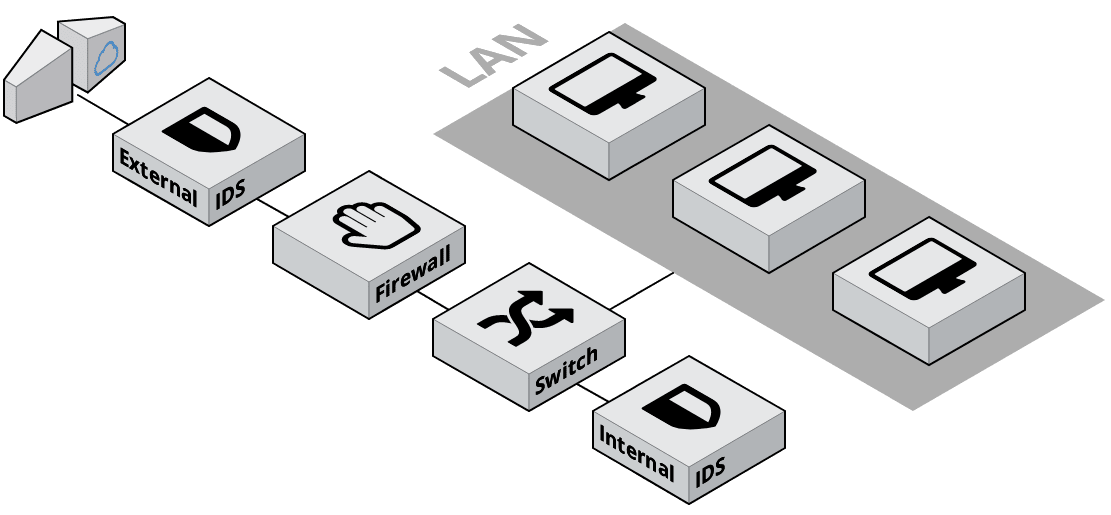
\includegraphics[scale=0.2]{assets/figures/chapter2/Intrusion Detection System Model.png}
        \caption{Intrusion Detection System Model}
        \label{fig:IDS-model}
\end{figure}
\noindent The functions demanded to an \gls{ids} are basically to detect and give information about threats, such as those discussed in \ref{subsec:malicious-traffic}. There is a variety of implementations of \glsplural{ids} and detection models, which are briefly discussed in the following section \ref{subsec:taxonomy-ids}.

%----------------------------------------------------
% TAXONOMY OF INTRUSION DETECTION SYSTEMS
%----------------------------------------------------

%See paper \cite{Liu2019}

\subsection{Taxonomy of Intrusion Detection Systems}
\label{subsec:taxonomy-ids}

Different researchers have developed multiple classification representations of \glsplural{ids}: they can be classified by source of data (either host or network based, or both), by detection technique (anomaly based, signature based, or can use artificial intelligence). A good summary of the taxonomy and methodologies used can be \cite{Hodo2017} and \cite{Liu2019}, which cover also \gls{ml} applied to \gls{ids}.

%----------------------------------------------------
% HIDS AND NIDS
%----------------------------------------------------

\subsubsection{HIDS and NIDS}
\label{subsubsec:hids-nids}

As mentioned above, \glsplural{ids} can fall into two different categories: \gls{hids} was the first type to be implemented \cite{Debar1999} and consists in an application that, once installed on a host machine, analyzes and monitors all the network activities related to such computer. The traffic activities gathered are called \textit{audit trails}. There is one main advantage in using this typology of \gls{ids}: being able to detect threats before sending and receiving data. Its main disadvantage is that in order to monitor the whole network, it would be necessary to install that piece of software in every host \cite{Hodo2017}, resulting in occupying resources and in depending on the reliability of the single host, which can be compromised in other ways \cite{Liu2019}. \\ On the other hand a \gls{nids} can be considered as a strong deterrence against outside intruders, in fact it is placed at specific points on the network (usually deployed on major hosts or switches), monitoring the network links. The main disadvantage is its weakness in detecting attacks generated inside the network \cite{Hodo2017}, because of its nature, it monitors only specific network segments \cite{Liu2019}.

%----------------------------------------------------
% ANOMALY BASED DETECTION
%----------------------------------------------------

\subsubsection{Anomaly-based Detection}
\label{subsubsec:anomaly-detection}

This is a behavioural-based technique that observes changes in normal activity by building, over a period of time, a profile of the monitored system. The main advantage of this technique is that it allows for unknown attack detection (since it knows what normal traffic looks like). \\ According to \cite{Hodo2017}, there are two categories of Anomaly Detection: \textit{self-learning} and \textit{programmed}. The first one is also divided in two branches: \textit{time series model}, that considers a sequence of observations in order of succession (heavily relying on probability analysis) and \gls{ml} that will be discussed in section \ref{sec:machine-learning}. Instead, a programmed model (divided into \textit{threshold}, \textit{simple rule based} and \textit{statistical models}) consists of a system that needs an external entity for learning how to detect changes in behaviour.

%----------------------------------------------------
% SIGNATURE-BASED DETECTION
%----------------------------------------------------

\subsubsection{Signature-based Detection}
\label{subsubsec:signature-detection}

Signature-based detection uses a set of pre-defined rules to match the patterns in the network traffic \cite{Hodo2017}. Its selling point is the low false-positive detection ratio, whereas its main drawback is the detection capabilities: stuck to the database of known attacks. For this reason this type of detection will not be considered in this project.

%----------------------------------------------------
% DATASETS FOR INTRUSION DETECTION SYSTEMS
%----------------------------------------------------

\subsection{Datasets for Intrusion Detection Evaluation}
\label{subsec:datasets-for-evaluation}

%See paper \cite{icissp18}, \cite{Khraisat2019} and \cite{Leevy2020}

\textit{Datasets} are fundamental in the developing stage of an \gls{ids} for testing purposes and performance evaluation. As pointed out in \cite{icissp18}, many researchers struggle to find a reliable and comprehensive dataset, that is also up to date regarding the attacks used to generate it, since there are datasets that date back to 1998. The timeline below represents major dataset releases, used in many different researches.

\begin{figure}[h!]
    \begin{center}
        \begin{chronology}*[2]{1998}{2021}{0.85\textwidth}
            \event{1998}{DARPA}
            \event{1999}{KDD}
            \event{2002}{DEFCON}
            \event{2016}{CAIDA}
            \event{2005}{LBNL}
            \event{2009}{CDX \\ Twente \\ Kyoto}
            \event{2011}{UMASS}
            \event{2012}{ISCX2012}
            \event{2013}{ADFA}
            \event{2017}{CICIDS2017}
            \event{2018}{CICIDS2018}
            \event{2021}{AWID3}
        \end{chronology}
    \end{center}
    \caption{Datasets timeline}
\end{figure}

\noindent The datasets relevant to this project, used for testing tools, algorithms\footnote{See chapter \ref{chap:methodology}} and understanding what a particular feature can tell about the flow are: 
\begin{itemize}
    \item[\faCaretRight] \textit{CICIDS2017}: developed in 2017 by the \gls{cic}, it is a good trade-off between complexity and weight. It consists of benign and malicious traffic (labeled), obtained from a lab environment over 5 days and containing the threats disclosed in section \ref{subsec:malicious-traffic}. It has more than 80 traffic feature per flow, provided in a \glsxtrshort{csv}, together with the \gls{pcap} files containing the traffic dump. The total size of this dataset is around 50 GB;
    \item[\faCaretRight] \textit{NSL-KDD}: this dataset is an improved version of the original KDD'99 \cite{Tavallaee2009} to address some of its shortcomings \cite{McHugh2000}. Although it can be anachronistic for the attacks considered since it is more than 20 years old, it is certainly useful and lightweight for understanding intrusion detection methods. The total size of this dataset is around 50 MB.
\end{itemize}

\noindent An alternative to take into consideration could be to create a custom dataset, acquiring traffic data wih software like \textit{Wireshark} \cite{WiresharkWebsite} and processing it to extract features and related statistics.

%----------------------------------------------------
% DETECTION RATES
%----------------------------------------------------

\subsection{Detection rates and base-rate fallacy}
\label{subsec:detection-rates}

Understanding how accurate is an \gls{ids}, or a detection model is fundamental for making the right choices during the development. Moreover, understanding which parameters are important and which may only \textit{seem} to be important. These values can be obtained using some probability calculation and statistics. In \cite{Axelsson2000} the author used, with this purpose, the \textit{base-rate fallacy}, one of the cornerstones of Bayesian statistics. A similar concept was applied in \cite{Liu2019} for evaluating the effectiveness of a \gls{ml} algorithm. The parameters needed to evaluate the \textit{effectiveness} of an \gls{ids} are:
\begin{itemize}
    \itemAR \gls{tp} \textit{rate}: namely, a measure of attacks rightly classified as threats. It is represented by the conditional probability of an alarm triggered $A$ given that there has been an intrusion $I$, so $P(A|I)$;
    \itemAR \gls{fp} \textit{rate}: also called \textit{False Alarm rate}, it indicates a measure of normal events, misclassified as attacks. It it the conditional probability of an attack being detected, given that there wasn't any, so $P(A|\neg I)$.
\end{itemize}
Recalling the \textit{conditional probability} of $A$, given that $B$ has occurred:
\begin{equation}
    P(A|B)=\frac{P(A)\cdot P(B|A)}{P(B)}
    \label{eq:conditional-prob}
\end{equation}
And the \textit{Bayes Theorem}:
\begin{equation}
    P(A|B)=\frac{P(A)\cdot P(B|A)}{\sum_{i=1}^nP(A_i)\cdot P(B|A_i)}
    \label{eq:Bayes-th}
\end{equation}
It is now possible to make some assumptions on what the ideal \gls{ids} should aim to: achieving substantial values of \textit{Bayesian Detection rate} $P(I|A)$, minimizing $P(A|\neg I)$, in other words, the false alarms. Considering \ref{eq:Bayes-th}, the Bayesian Detection rate can be calculated:
\begin{equation}
    P(I|A)=\frac{P(I)\cdot P(A|I)}{P(I)\cdot P(A|I)+ P(\neg I)\cdot P(A|\neg I)}
    \label{eq:Bayesian-detection-rate}
\end{equation}
Equation \ref{eq:Bayesian-detection-rate} refers to the probability that an alarm really indicates an intrusion: it is noticeable now that the limiting-factor in an \gls{ids} is not the ability to identify the behaviour correctly as a threat, rather its ability to suppress false alarms: the factor concerning the detection rate is overshadowed by the factor governing the false alarm rate, since intrusions don't happen so often, $P(I)<P(\neg I)$, but it is also true that $P(I)+P(\neg I)=1$; giving some examples for further explanation, assuming $P(I)=2\cdot 10^{-5}\Rightarrow P(\neg I)=0.99998$, and now the discrepancy is evident \cite{Axelsson2000}. \\ This demonstrates that, during the development of an \gls{ids} it is necessary to keep an eye on the \gls{fp} \textit{rate}, in order to be as effective as possible.

%----------------------------------------------------
% MACHINE LEARNING
%----------------------------------------------------

\section{Machine Learning}
\label{sec:machine-learning}

%See paper \cite{Khraisat2019} and \cite{Hodo2017} \\

\glsreset{ml} \gls{ml} can be defined as computational methods using \textit{experience} to improve performance or to make accurate predictions \cite{Mohri2018}. Here experience has to be intended as information available to the learner.

%----------------------------------------------------
% LEARNING SCENARIOS
%----------------------------------------------------

\subsection{Learning scenarios}
\label{subsec:learning-scenarios}

Learning scenarios differ in the types of training data used, the order and the method by which it is received by the learner. Some common scenarios, useful for the treatment of this project are:

%----------------------------------------------------
% SUPERVISED LEARNING
%----------------------------------------------------

\subsubsection{Supervised Learning}
\label{subsubsec:supervised-learning}

The learner receives a set of labeled examples as training data and makes predictions for all unseen points. This is the most common scenario associated with classification, regression and ranking problems \cite[p. 6]{Mohri2018}. This type of approach usually consists of two stages: \textit{training} and \textit{testing} \cite{Khraisat2019}. During the former, relevant features and classes are identified and then the algorithm learns from this data samples. Referring to this project, an \gls{ids} that uses supervised learning uses records containing a network or host data source and a label, namely, for example, \textit{normal} or \textit{malicious}. The goal, in this case, is to train a classifier using supervised learning technique, to learn the inherent relationship between the input data and the labelled output value.

%----------------------------------------------------
% UNSUPERVISED LEARNING
%----------------------------------------------------

\subsubsection{Unsupervised Learning}
\label{subsubsec:unsupervised-learning}

Unlike the previous scenario, the learner exclusively receives unlabeled training data, and makes predictions for all unseen points. It can be difficult to evaluate the performance of a learner using this methodology \cite[p. 6]{Mohri2018}. In unsupervised learning no labels are given, and instead the data is grouped automatically into various classes through the learning process: the \textit{k-means technique} is one of the most prevalent techniques of \textit{clustering analysis} (grouping objects into subsets with meaning in the context of a particular problem \cite{Annachhatre2015}) that aims to separate $n$ data objects into $k$ clusters. Each data object is assigned by the cluster with the nearest mean. The number of clusters is decided by the user, for example, each cluster can represent a particular behaviour to detect.

%----------------------------------------------------
% REINFORCEMENT LEARNING
%----------------------------------------------------

\subsubsection{Reinforcement Learning}
\label{subsubsec:reinforcement-learning}

In contrast with the other two scenarios, the reinforcement learning one involves multiple rounds where training and testing phases are intermixed. To collect information, the learner actively interacts with the environment and in some cases affects it, receiving an immediate reward for each action. The goal of the learner is to maximize his reward over a course of actions and iterations with the environment \cite[p. 7]{Mohri2018}. The learner is faced with the \textit{exploration versus exploitation dilemma}, since he must choose between exploring unknown actions to gain more information or exploiting the information already collected. The autonomous agent must lean to perform a task by trial and error, without any guidance from the human operator \cite[p. 25]{Goodfellow2016}.

%----------------------------------------------------
% MACHINE LEARNING ALGORITHMS
%----------------------------------------------------

\subsection{Machine Learning Algorithms}
\label{subsec:ml-algorithms}

\faEdit\quad \textbf{To be discussed with Supervisor: supervised vs reinforcement learning} \\

\textcolor{dimgray}{\lipsum[1-4]}

%----------------------------------------------------
% DEEP LEARNING
%----------------------------------------------------

\subsection{Deep Learning}
\label{subsec:deep-learning}

\textcolor{dimgray}{\lipsum[1-3]}

%----------------------------------------------------
% MACHINE LEARNING LIBRARIES
%----------------------------------------------------

\subsection{Machine Learning Libraries}
\label{subsec:ml-libraries}

\textcolor{dimgray}{\lipsum[1]}